\documentclass{standalone}
\usepackage{tikz}

\begin{document}
 	\begin{tikzpicture}
 		\draw (0, 0) node[opacity=0.7] {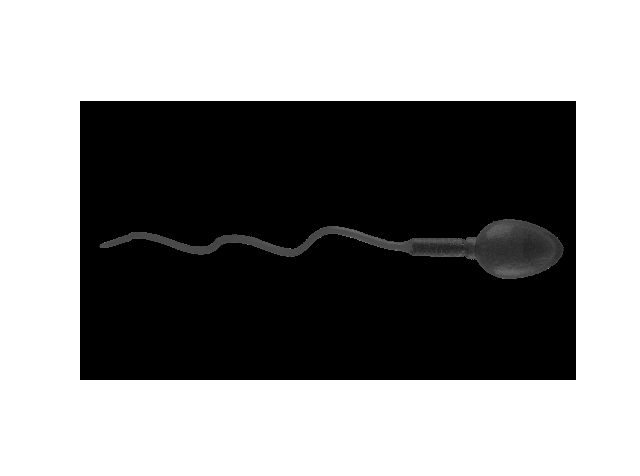
\includegraphics{images/original_gs_2.png}};
		\draw[help lines, color=gray!30, dashed] (-7,-4) grid (7,4);
		\draw[->,ultra thick] (-7.2,0)--(7.2,0);% node[right]{$x$};
		\draw[->,ultra thick] (0,-5)--(0,5);% node[above]{$y$};
		
		
   		
   		\draw(15,0) node {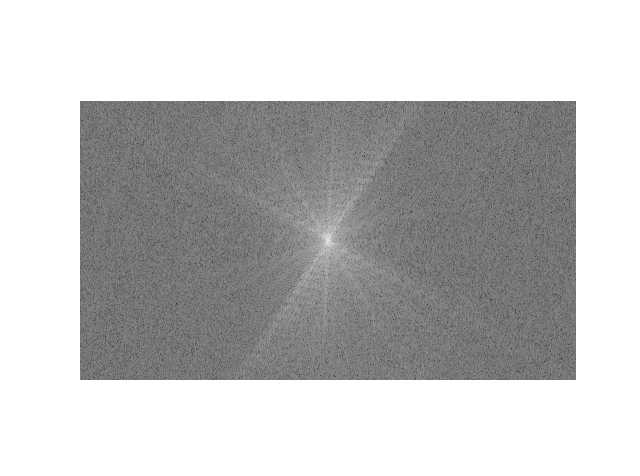
\includegraphics{images/fourier_domain.png}};
		\draw[help lines, color=gray!30, dashed] (8,-4) grid (22,4);
		\draw[->,ultra thick] (7.8,0)--(22.2,0);% node[right]{$\alpha$};
		\draw[->,ultra thick] (15,-5)--(15,5);% node[above]{$\omega$};
		\draw[ultra thick, color=red!20!white] (11,4)--(19,-4);
		%\draw[ultra thick, color=red!20!white] (-1,8)--(7,0);
		
		%\draw[ultra thick, color=red!20!white] (-1,8)--(-12,-4);
		%\draw[ultra thick, color=red!20!white] (3,4)--(-4,-4);
		%\draw[ultra thick, color=red!20!white] (7,0)--(4,-4);
		
		
		\coordinate (a) at (2,-5);
		\coordinate (b) at (13,-5);
		\draw[->, >=latex, red!20!white, line width=15pt]   (a) to node[black]{2D Fourier transform} (b) ;
		
		\draw(5,4) node[opacity=0.5] {
\includegraphics{images/path.png}};
		
		\coordinate (d) at (2,5);
		\coordinate (e) at (13,5);
		\draw[->, >=latex, red!20!white, line width=15pt]   (d) to node[black]{1D Fourier slice} (e) ;
		
 	\end{tikzpicture}
\end{document}
